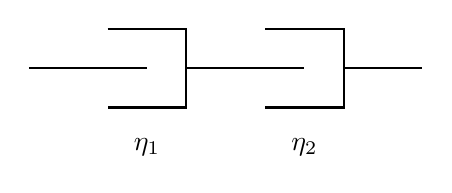
\begin{tikzpicture}
%\draw[fill=gray!23,gray!23](0,0) rectangle (7,4);
%\draw[step=0.5cm,gray,very thin] (0,0) grid (7,4); %background grid

\draw[thick] (0.5,2.5) -- (2,2.5) ;  
\draw[thick] (2.5,2.5) -- (4,2.5) ;  
\draw[thick] (4.5,2.5) -- (5.5,2.5) ;  

\draw[thick] (1.5,3) -- (2.5,3) -- (2.5,2) -- (1.5,2);  
\draw[thick] (3.5,3) -- (4.5,3) -- (4.5,2) -- (3.5,2);  

\node[] at (2,1.5) {$\eta_1$};
\node[] at (4,1.5) {$\eta_2$};

%--------------------------------------------------------
%\draw[thick] (1,1) -- (3,1.2) -- (2.7,3) -- (1.1,3.1) -- cycle;  
%\node[] at (0.8,0.8) {0};
%\node[] at (3.2,1) {1};
%\node[] at (2.9,3.1) {2};
%\node[] at (0.9,3.2) {3};
%\draw[black,fill=black] (1,1)     circle (2pt); \draw (1,1) circle (4pt);
%\draw[black,fill=black] (3,1.2)   circle (2pt); \draw (3,1.2) circle (4pt);
%\draw[black,fill=black] (2.7,3)   circle (2pt); \draw (2.7,3) circle (4pt);
%\draw[black,fill=black] (1.1,3.1) circle (2pt); \draw (1.1,3.1) circle (4pt);
%\draw[black,fill=black] (3.1,0.2) circle (2pt); \node[] at (3.4,0.2) {$\vec\upnu$};
%\draw (4.1,0.2) circle (4pt); 
%\node[] at (2.5,4.5) {4 vel. nodes, 4 press. nodes};
\end{tikzpicture}\\
